\section{Технический проект}
\subsection{Общая характеристика организации решения задачи}

Необходимо спроектировать и разработать приложение, который должен способствовать популяризации ролевых игр.

Приложение представляет собой набор взаимосвязанных различных окон, которые сгруппированы по разделам, содержащие текстовую, графическую информацию. Приложение располагается на компьютере.

\subsection{Обоснование выбора технологии проектирования}

На сегодняшний день информационный рынок, поставляющий программные решения в выбранной сфере, предлагает множество продуктов, позволяющих достигнуть поставленной цели – разработки приложения.

\subsubsection{Описание используемых технологий и языков программирования}

В процессе разработки приложения используются программные средства и языки программирования. Каждое программное средство и каждый язык программирования применяется для круга задач, при решении которых они необходимы.

\subsubsection{Язык программирования Python}

Python –  высокоуровневый язык программирования общего назначения с динамической строгой типизацией и автоматическим управлением памятью, ориентированный на повышение производительности разработчика, читаемости кода и его качества, а также на обеспечение переносимости написанных на нём программ. Язык является полностью объектно-ориентированным в том плане, что всё является объектами. Необычной особенностью языка является выделение блоков кода отступами. Синтаксис ядра языка минималистичен, за счёт чего на практике редко возникает необходимость обращаться к документации. Сам же язык известен как интерпретируемый и используется в том числе для написания скриптов. Недостатками языка являются зачастую более низкая скорость работы и более высокое потребление памяти написанных на нём программ по сравнению с аналогичным кодом, написанным на компилируемых языках, таких как C или C++.

Python — это язык программирования, который широко используется в интернет-приложениях, разработке программного обеспечения, науке о данных и машинном обучении (ML). Разработчики используют Python, потому что он эффективен, прост в изучении и работает на разных платформах. Программы на языке Python можно скачать бесплатно, они совместимы со всеми типами систем и повышают скорость разработки.

\subsubsection{Использование библиотеки Tkinter на Python}
	
\paragraph{Введение}
Библиотека Tkinter - это стандартная библиотека Python для создания графического пользовательского интерфейса (GUI). Она обладает широкими возможностями для создания разнообразных приложений с использованием различных виджетов, таких как кнопки, поля ввода, метки и многое другое.
	
\paragraph{Возможности Tkinter}
Вот некоторые из основных возможностей, предоставляемых библиотекой Tkinter:
	
\begin{enumerate}
	\item Создание различных виджетов: кнопки, метки, поля ввода, списки и многое другое.
	\item Управление компоновкой виджетов с использованием менеджеров компоновки (например, grid, pack, place).
	\item Обработка событий, таких как щелчок мыши, нажатие клавиш и другие.
	\item Возможность создания различных диалоговых окон, таких как окна предупреждений, информационные окна и окна запроса.
	\item Поддержка многопоточности для обновления интерфейса из различных потоков выполнения.
\end{enumerate}

\paragraph{Соединение движка и окон tkinter}
Модуль graphics содержит в себе библиотеку tkinter . Класс Graphics внутри модуля является наследником tk.Canvas. Этот класс взаимодействует с окном root = tk.TK() в программном модуле пользователя. Модуль sprite тоже взаимодействует с tkinter. Изображение для спрайта берётся с помощью метода tk.PhotoImage(file=name)
Пример представлен на рисунке \ref{tk:image}:
\begin{figure}[H]
	\begin{lstlisting}[language=Python]
		модуль sprite
		
		import tkinter as tk
		class Sprite:
			def __init__(self, image):
				self.image = tk.PhotoImage(file=image)
				self.tag = None
				self.x = 0
				self.y = 0
				self.z = 0		
				def set_tag(self, tag):
				self.tag = tag
			
			def set_z(self, z):
				self.z = z
			
			def get_tag(self):
				return self.tag	
			def set_coords(self, new_x, new_y):
				if self.tag:
				self.x = new_x
				self.y = new_y
			def update(self):
				pass
	\end{lstlisting}  
	\caption{Пример использования tkinter в программе}
	\label{tk:image}
\end{figure}
Продолжение на рисунке \ref{tkinter2:image}:
\begin{figure}[H]
	\begin{lstlisting}[language=Python]
		import tkinter as tk
		class Graphics(tk.Canvas):
			canvas = None
			def __init__(self, master, **kwargs):
				super().__init__(master, **kwargs)
				self.sprites = []
				Graphics.canvas = self			
			def add_sprite(self, sprite, x, y, z, **kwargs):
				tag = self.create_image(x, y, image=sprite.image, anchor='center', **kwargs)
				sprite.set_tag(tag)
				sprite.set_z(z)
				sprite.x = x
				sprite.y = y
				self.sprites.append(sprite)
				self.sprites.sort(key=lambda sprite: sprite.z)
			def update(self):
				for sprite in self.sprites:
					sprite.update()
					self.tag_raise(sprite.get_tag())
					self.coords(sprite.get_tag(), sprite.x, sprite.y)
					self.itemconfig(sprite.get_tag(), image=sprite.image)
					def change_sprite(self, sprite, new_sprite):
					old\_sprite_pos = None
				for i, s in enumerate(self.sprites):
					if s.get\_tag() == sprite.get_tag():
						old_sprite_pos = i
						break
				if old_sprite_pos is not None:
					old_tag = sprite.get_tag()
			
				self.sprites[old_sprite_pos] = new_sprite
				new_sprite.set\_tag(old_tag)
				new_sprite.set_tag(old_tag)
				new_sprite.set_z(sprite.z)
				self.tag_raise(old_tag)
				self.coords(old\_tag, sprite.x, sprite.y)
				self.itemconfig(old\_tag, image=new_sprite.image)
			
			def delete_sprite(self, sprite):
				self.delete(sprite.get_tag()
				self.sprites.remove(sprite)
			def clear_all(self):	
				for sprite in self.sprites:
					self.delete(sprite.get_tag())
					self.sprites.clear()
	\end{lstlisting}  
	\caption{Пример использования tkinter в программе}
	\label{tkinter2:image}
\end{figure}


Продолжение на рисунке \ref{tkinter3:image}:
\begin{figure}[H]
	\begin{lstlisting}[language=Python]
		модуль baldursgame '''пользовательский модуль'''
		from ruins import *
		from village import *
		import time
		import random
		class BaldursGame(Game):
		def __init__(self, canvas, window, **params):
		super().__init__(canvas, window, **params)
		from mage import Mage
		self.add_pc_to_team(Mage(0, 0, 0))
		self.new_area('Ruins', Ruins())
		self.new_area('Village', Village())
		self.set_area('Ruins')
		self.set_team(500, 300, 100)
		self.timer()
		модуль main
		from bggame import *
		root = tk.Tk()
		root.geometry('1500x1500')
		exit_button = tk.Button(root, text="Exit", fg="red", command=root.destroy)
		canvas = Graphics(root, width=1500, height=1500)
		Graphics.canvas = canvas
		BaldursGame(canvas, root)
		canvas.place(height = 1500, width =1500)
		BaldursGame.timer
		root.mainloop()
	\end{lstlisting}  
	\caption{Пример использования tkinter в программе}
	\label{tkinter3:image}
\end{figure}
	
\paragraph{Заключение}
Библиотека Tkinter предоставляет мощные инструменты для создания графических пользовательских интерфейсов на языке Python. Реализация таймеров на Python может быть достигнута с помощью модулей \texttt{time} или \texttt{threading}, в зависимости от конкретных требований приложения.


\subsection{Архитектура платформы для создания ролевых игр}
\subsubsection{Диаграмма компонентов классов}
Диаграмма компонентов описывает особенности физического представления разрабатываемой системы. Она позволяет определить архитектуру системы, установив зависимости между программными компонентами, в роли которых может выступать как исходный, так и исполняемый код. Основными графическими элементами диаграммы компонентов являются компоненты, интерфейсы, а также зависимости между ними. На рисунке \ref{diagram:image} изображена диаграмма компонентов для проектируемой системы. Она включает в себя основной класс платформы игры Game и производные от него классы, класс Object с наследниками и их параметрами (полями и методами).
\begin{figure}[ht]
	\center{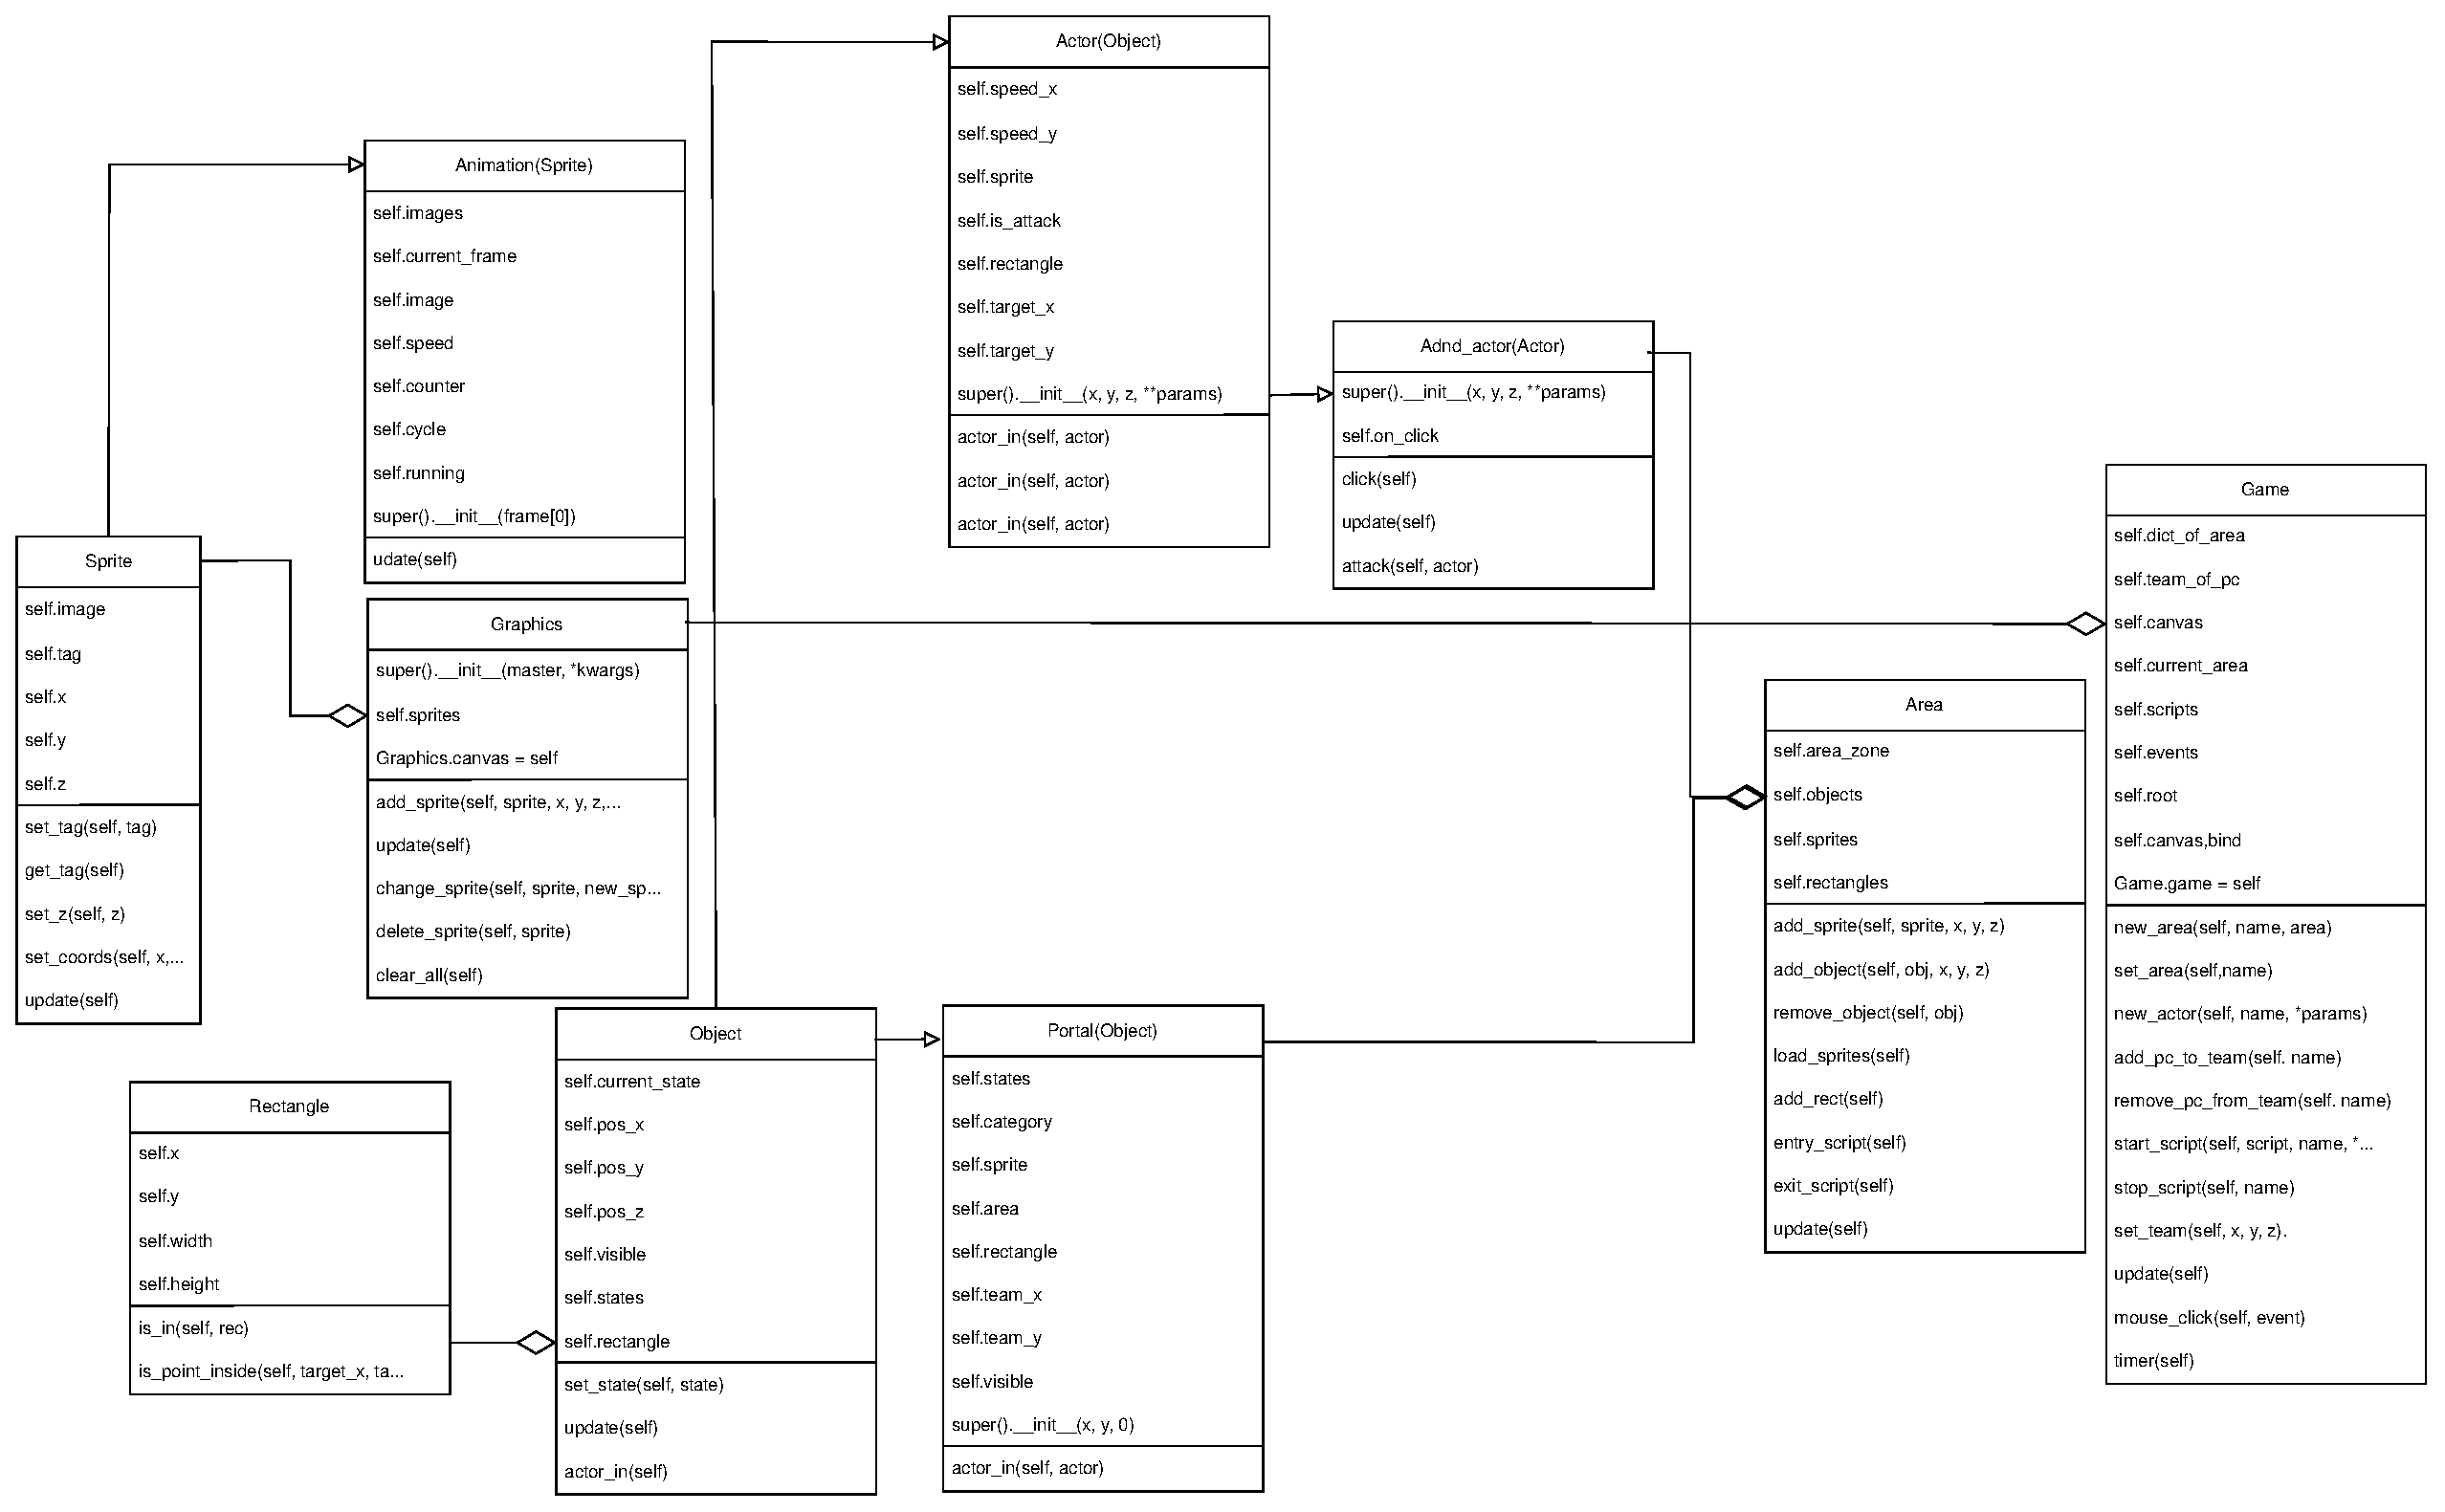
\includegraphics[width=1\linewidth]{diagram}}
	\caption{Диаграмма компонентов}
	\label{diagram:image}
\end{figure}
\paragraph{Описание классов}
	Graphics -- класс, управляющий спрайтами. Содержит в себе следующие поля:
		self.sprites -- список спрайтов. И методы:
		\begin{enumerate}
			\item add\_sprite(self, sprite x, y, z, image) -- добавляет в список спрайт, сохраняет координаты.
			\item change\_sprite(self, sprite new\_sprite) -- меняет местами спрайты в списке.
			\item delete\_sprite(self, sprite) -- удаляет спрайт из списка.
			\item clear\_all(self) -- очищает список спрайтов.
			\item update(self) -- добавляет все спрайты из списка на форму.
		\end{enumerate}
	Sprite -- класс, хранящий в себе изображение игровых объектов image. Содержит в себе следующие поля:
		\begin{enumerate}
			\item self.x -- координата x.
			\item self.y -- координата y.
			\item self.z -- координата z.
			\item self.tag -- уникальный номер спрайта.
			\item self.image -- изображение.
		\end{enumerate}
		И методы:
		\begin{enumerate}
			\item set\_tag(self, tag) -- устанавливает tag спрайту.
			\item get\_tag(self) -- возвращает tag спрайта.
			\item set\_z(self, z) -- устанавливает z координату.
			\item set\_coords(self, new\_x, new\_y) -- устанавливает новые координаты.
			\item update(self) -- ничего не делает.
		\end{enumerate}
	Animation -- класс, хранящий в себе список изображений игровых объектов image. Потомок класса Sprite.  Содержит в себе следующие поля:
		\begin{enumerate}
			\item self.current\_frame -- текущий кадр.
			\item self.images  -- Загрузка всех кадров анимации.
			\item self.image -- Установка начального изображения.
			\item self.speed -- скорость анимации.
			\item self.counter -- счётчик кадров.
			\item self.cycle -- проверка на то что должна ли быть анимация циклично или нет.
			\item self.running -- проверка проигрывается ли сейчас анимация.
			\item update(self) -- обновляет кадр в анимации.
		\end{enumerate}
		И метод: update(self) -- обновляет кадр в анимации.
	Rectangle -- абстрактный класс прямоугольника. Содержит в себе следующие поля:
		\begin{enumerate}
			\item self.pos\_x -- координата x.
			\item self.pos\_y -- координата y.
			\item self.width -- ширина.
			\item self.height -- высота.
		\end{enumerate}
		И методы:
		\begin{enumerate}
			\item is\_in(self, rect) -- функция проверки нахождения одного прямоугольника в другом.
			\item is\_point\_inside(self, target\_x, target\_y) -- функция проверки точки в пределах прямоугольника.
		\end{enumerate}
	Object -- класс, от которого наследуются классы Adnd\_Actor, Actor, Portal. Содержит в себе следующие поля:
		\begin{enumerate}
			\item self.pos\_x -- координата x.
			\item self.pos\_y -- координата y.
			\item self.pos\_z -- координата z.
			\item self.current\_state -- текущее состояние.
			\item self.visible -- видимость портала.
			\item self.on\_click -- функция клика по объекту.
			\item self.rectangle -- прямоугольник объекта.
		\end{enumerate}
		И методы:
		\begin{enumerate}
			\item set\_state(self, state\_name) -- устанавливает состояние.
			\item actor\_in(self, actor) -- ничего не делает.
			\item update(self) -- ничего не делает.
		\end{enumerate}
	Portal -- класс объекта для перехода между зонами. Потомок класса Object. Содержит в себе следующие поля:
		\begin{enumerate}
			\item self.states -- состояние портала.
			\item self.sprite -- спрайт портала.
			\item self.category -- категория.
			\item self.rectangle -- прямоугольник портала.
			\item self.area -- зона в которую ведёт портал.
			\item self.team\_x -- координата x в  которую нужно разместить команду.
			\item self.team\_y -- координата y в  которую нужно разместить команду.
			\item self.visible -- видимость портала.
		\end{enumerate}
		И методы:
			actor\_in(actor) -- события, которые произойдут, когда персонаж окажется внутри прямоугольника портала.
	Actor -- класс персонажа, содержащий внутри себя основные поля и методы для перемещения по рабочему окну. Содержит в себе следующие поля:
		\begin{enumerate}
			\item self.sprite -- спрайт персонажа.
			\item self.speed\_x -- значение скорости x.
			\item self.speed\_y -- значение скорости y.
			\item self.target\_x -- координата x в которую должен прийти персонаж.
			\item self.target\_y -- координата y в которую должен прийти персонаж.
			\item self.rectangle -- прямоугольник персонажа.
			\item self.is\_attack -- атакует ли сейчас персонаж.
		\end{enumerate}
		И методы:
		\begin{enumerate}
			\item update(self) -- функция обновления координат и состояния персонажа.
			\item search\_position(self, new\_x, new\_y) -- поиск координат в которые нужно двигаться персонажу.
			\item stop\_move(self) -- остановка движения персонажа.
		\end{enumerate}
	Adnd\_Actor -- класс персонажа, содержащий методы связанные с взаимодействием с другими персонажами. Является наследником Actor. Содержит в себе следующие поля:
		self.on\_click событие при клике на персонажа
		И методы:
		\begin{enumerate}
			\item update(self) -- функция обновления координат и состояния персонажа.
			\item click(self) -- функция вызывается при клике по персонажу.
			\item attack(self, actor) --  функция атаки персонажа по другому персонажу.
		\end{enumerate}
	Area -- зона, в которой находятся персонажи и объекты. Содержит следующие поля:
		\begin{enumerate}
			\item self.area\_zone -- параметр определяющий особенности конкретной зоны.
			\item self.objects -- список, хранящий в себе множество объектов.
			\item self.sprites -- список фоновых спрайтов.
			\item self.rectangles -- прямоугольник зоны.
		\end{enumerate}
		И методы:
		\begin{enumerate}
			\item add\_sprite(self, sprite, x, y, z) -- функция добавляет спрайт в зону.
			\item add\_object(self, obj, x, y, z) -- функция добавляет объект в зону.
			\item remove\_object(self, obj) -- функция удаляет объект из зоны.
			\item load\_sprites(self) -- функция загружает все спрайты зоны.
			\item add\_rect(self, rec) -- функция добавляет прямоугольник в зону.
			\item entry\_script(self) -- функция запускается, когда команда входит в зону.
			\item exit\_script(self) -- функция запускается, когда команда выходит из зоны.
			\item update(self) -- функция изменяет и проверяет изменение всех объектов в зоне.
		\end{enumerate}
	Game -- класс, управляющий игровой системой. Имеет следующие поля:
		\begin{enumerate}
			\item self.rpg\_dict\_of\_area -- словарь, хранящий в себе множество экземпляров класса Area.
			\item self.team\_of\_pc -- список, хранящий в себе имена экземпляров класса Actor с параметром category = "pc".
			\item self.canvas -- графика.
			\item self.root -- окно для графики.
			\item self.current\_area -- параметр хранящий, текущую зону.
			\item self.scripts -- словарь для хранения запущенных сценариев.
			\item self.events -- словарь для хранения запущенных event`ов сценариев.
			\item self.canvas.bind("<Button-1>", self.mouse\_left.\_click) -- обработка клика мыши по рабочему окну.
		\end{enumerate}
		И методы:
		\begin{enumerate}
			\item new\_area(self, name, area) -- функция добавляет новую зону в список.
			\item set\_area(self, name) -- функция устанавливает текущую зону, загружает графику зоны.
			\item new\_actor(self, name, **params) -- функция создаёт класс, потомок от Actor и создаёт поле из параметров, и установление их в начальные значения.
			\item add\_pc\_to\_team(self, pc) -- функция добавляет персонажа в команду.
			\item remove\_pc\_from\_team(self, pc) -- функция удаляет персонажа из команды.
			\item start\_script(self, script\_function, script\_name, *args) -- функция запускает сценарий в отдельном потоке с возможностью остановки и передачи аргументов.
			\item stop\_script(self, script\_name) -- функция останавливает сценарий по имени.
			\item set\_team(self, x, y, z) -- функция устанавливает координаты персонажей команды.
			\item update(self) -- функция вызывается в таймере для обновления всех переменных в текущей зоне.
			\item mouse\_left\_click(self, event) -- функция обрабатывает клик мыши.
			\item timer(self) -- функция должна вызывать метод update постоянно.
		\end{enumerate}

\subsubsection{Реализация графической подсистемы}
Графическая подсистема основана на библиотеке tkinter, которая используется для создания графического интерфейса пользователя. В контексте платформы, tkinter используется для отображения и управления спрайтами — графическими объектами, которые представляют персонажей, предметы и другие элементы игры.
\paragraph{Система спрайтов}
Она реализована через класс Graphics, который расширяет tk.Canvas. Этот класс управляет отображением спрайтов на холсте, их сортировкой по z-координате (что позволяет создать эффект глубины), а также обновлением их позиций. Спрайты могут быть добавлены, перемещены и удалены с холста. Вот пример метода, который добавляет спрайт на холст:
Пример на рисунке \ref{ttk:image}:
\begin{figure}[H]
	\begin{lstlisting}[language=Python]
		def add\_sprite(self, sprite, x, y, z, **kwargs):
			tag = self.create\_image(x, y, image=sprite.image, anchor='center', **kwargs)
			sprite.set\_tag(tag)
			sprite.set\_z(z)
			self.sprites.append(sprite)
			self.sprites.sort(key=lambda sprite: sprite.z)
\end{lstlisting}  
\caption{Пример добавления спрайта на холст}
\label{ttk:image}
\end{figure}
\subsubsection{Реализация зон}
Зоны в программе представляют собой различные игровые области. Каждая зона реализована через класс Area, который содержит спрайты и объекты, принадлежащие этой зоне. Класс Area является ключевым элементом в структуре игры, так как он определяет отдельные игровые зоны, которые игрок может исследовать. Каждая зона представляет собой уникальный участок игрового мира со своим набором характеристик и поведения.

Спрайты и объекты: В основе каждой зоны лежат спрайты и объекты. Спрайты — это графические элементы, такие как персонажи, враги или декорации, которые игрок видит на экране. Объекты могут быть как видимыми, так и невидимыми элементами, которые взаимодействуют с игроком или окружением, например, триггеры событий или коллекционные предметы.
Скрипты входа и выхода: entry\_script и exit\_script — это скрипты, которые активируются при входе игрока в зону и при выходе из неё соответственно. Эти скрипты могут использоваться для запуска кат-сцен, начала битв, обновления заданий или любых других событий, которые должны произойти при изменении зоны.
Метод update: Метод update вызывается каждый игровой цикл и отвечает за обновление состояния всех спрайтов и объектов в зоне. Это может включать анимацию спрайтов, проверку столкновений, выполнение игровой логики и многое другое. Если в зоне заданы скрипты входа или выхода, метод update также будет их вызывать в соответствующий момент.
В целом, класс Area обеспечивает структурированное и модульное построение игрового мира, позволяя разработчикам создавать сложные и интерактивные зоны, которые делают игровой процесс более разнообразным и захватывающим. Это также упрощает управление ресурсами и оптимизацию, так как каждая зона может быть загружена и выгружена независимо от остальных.
\subsubsection{Реализация объектов и персонажей}
Объекты и персонажи являются ключевыми элементами игрового мира. Они реализованы через классы Object и Adnd\_Actor соответственно. Object может представлять любой игровой объект, который может взаимодействовать с игроком или окружением. Adnd\_Actor расширяет Object и добавляет дополнительные свойства и методы, специфичные для персонажей, такие как движение, атака и взаимодействие с другими персонажами.
Класс Object служит основой для всех элементов в игре, которые могут взаимодействовать с игроком или средой. Это могут быть предметы, такие как ключи, оружие, сундуки с сокровищами, или даже более абстрактные понятия, такие как ловушки или интерактивные точки.
Класс Adnd\_Actor расширяет Object, добавляя свойства и методы, которые специфичны для персонажей игры. Это включает в себя движение, атаку, взаимодействие с другими персонажами и возможность реагировать на изменения в игровой среде.
Эти классы позволяют разработчикам игр создавать разнообразные и динамичные объекты и персонажи, каждый из которых обладает уникальными характеристиками и способностями. Объекты могут быть простыми и служить одной цели, например, быть предметом для сбора, или же могут быть сложными, выполняя ряд функций в игре. Персонажи, с другой стороны, являются более сложными сущностями, которые могут взаимодействовать с игроком и другими элементами игрового мира на более глубоком уровне, выполняя различные действия, такие как бой, торговля или выполнение заданий.
\subsubsection{Реализация сценариев}
Сценарии в игре используются для создания интерактивных и динамических событий. Они могут быть реализованы как функции, которые запускаются в отдельных потоках, позволяя игре продолжать обрабатывать другие задачи в фоновом режиме. Класс Game содержит методы start\_script и stop\_script для управления этими сценариями. Thread – это отдельный поток выполнения. Это означает, что в программе могут работать две и более подпрограммы одновременно. Но разные потоки на самом деле не работают одновременно: это просто кажется.
Соблазнительно думать, что в программе работают два (или более) разных процессора, каждый из которых выполняет независимую задачу одновременно. Это почти правильно, но это то, что обеспечивает многопроцессорность (multiprocessing).
Запуск потоков (threading) похожа на эту идею, но ваши программы работает только на одном процессоре. Различные задачи, внутри потоков выполняются на одном ядре, а операционная система управляет, когда программа работает с каким потоком.
Поскольку потоки выполняется на одном процессоре, они хорошо подходят для ускорения некоторых задач, но не для всех. Задачи, которые требуют значительных вычислений ЦП и тратят мало времени на ожидание внешних событий, очевидно используя многопоточность не будут выполняться быстрее, вместо этого следует использовать многопроцессорность (multiprocessing).

Архитектура программы при использования многопоточности также может помочь в достижении более чистой архитектуры проекта. Использование потоков поможет сделать их архитектуру чище и понятнее.
Потоки (Thread)
Стандартная библиотека Python предоставляет библиотеку threading, которая содержит необходимые классы для работы с потоками. Основной класс в этой библиотеки Thread. Чтобы запустить отдельный поток, нужно создать экземпляр потока Thread и затем запустить его с помощью метода .start(). Пример на рисунке \ref{treading:image}:
\begin{figure}[H]
	\begin{lstlisting}[language=Python]
		import threading
		import time
		def thread_function(name):
			logging.info("Thread %s: starting", name)
			time.sleep(2)
			logging.info("Thread %s: finishing", name)
		if __name__ == "__main__":
			format = "%(asctime)s: %(message)s"
			logging.basicConfig(format=format, level=logging.INFO,
			datefmt="%H:%M:%S")
			logging.info("Main    : before creating thread")
			x = threading.Thread(target=thread_function, args=(1,))
			logging.info("Main    : before running thread")
			x.start()
			logging.info("Main    : wait for the thread to finish")
			# x.join()
			logging.info("Main    : all done")
		x = threading.Thread(target=thread_function, args=(1,))
		x.start()
	\end{lstlisting}  
	\caption{Пример метода tread.start}
	\label{treading:image}
\end{figure}
Когда создается поток Thread, ему передается функцию и список, содержащий аргументы этой функции. В примере указывается Thread, чтобы он запустил функцию thread\_function() и передаем ему 1 в качестве аргумента.

Сама по себе функция thread\_function() мало что делает. Она просто выводит некоторые сообщения с промежутком time.sleep() между ними.
Демоны потоков.
В информатике daemon (демон) – это процесс, который работает в фоновом режиме.

Python потоки имеет особое значение для демонов. Демон потока (или как еще его можно назвать демонический поток) будет остановлен сразу после выхода из программы. Один из способов думать об этих определениях – считать демон потока как потоком, который работает в фоновом режиме, не беспокоясь о его завершении.

Если в программе запущены потоки, которые не являются демонами, то программа будет ожидать завершения этих потоков, прежде чем сможет завершится. Тем не менее, потоки, которые являются демонами, при закрытие программы просто убиваются, в каком бы они состояние ни находились.
join()
Чтобы указать одному потоку дождаться завершения другого потока, вам нужно вызывать .join().  Если вызвать .join(), этот оператор будет ждать, пока не завершится любой вид потока.
\subsubsection{Вычисление пересечения прямоугольников}
Для определения столкновений и взаимодействий между объектами используется класс Rectangle. Он содержит методы, такие как is\_in, который проверяет, находится ли один прямоугольник внутри другого, и is\_point\_inside, который проверяет, находится ли точка внутри прямоугольника. Вот пример метода is\_point\_inside на рисунке \ref{tttk:image}:
\begin{figure}[H]
	\begin{lstlisting}[language=Python]
		def is\_point\_inside(self, target\_x, target\_y):
		return (self.x <= target\_x <= self.x + self.width) and
		(self.y <= target\_y <= self.y + self.height)
		Этот метод использует логические операторы для проверки, находится ли точка (target\_x, target\_y) в пределах прямоугольника, определенного координатами (x, y) и размерами (width, height).
\end{lstlisting}  
\caption{Пример метода is\_point\_inside класса Rectangle}
\label{tttk:image}
\end{figure}

